\section{宏观力学和运动学综合}
\subsection{综合例题1}
\paragraph{例1}\ \ \ \ 一弧形轨道AB如图6-1,最高点A的高度为$h$.其上任意一点C,满足该点高度$h_C=h_1,\rho_C=h^2_1+\rho_0$,其中$\rho_C$为C点曲率半径,$\rho_0$为轨道最低点B点曲率半径.一质量为$m$的小球从A点静止释放,问当小球与轨道间的摩擦系数$\mu$取何值时,小球下落到B点再次静止?\\\begin{wrapfigure}{r}{3.5cm}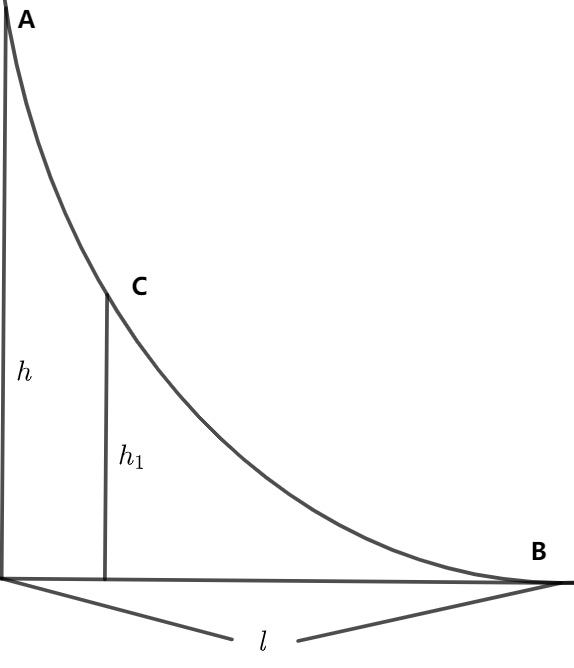
\includegraphics[width=3.5cm]{6-1}\end{wrapfigure}
	
\subsection{综合习题1}